\documentclass[12pt]{article}
\renewcommand{\baselinestretch}{1.8}

\usepackage[b4paper]{geometry}
\usepackage{tikz-qtree}
\usepackage{algorithm}
\usepackage{algpseudocode}
\makeatletter
\renewcommand{\ALG@beginalgorithmic}{\footnotesize}
\makeatother
\usepackage{graphicx}
\usepackage{subcaption}
\usepackage{showkeys}
\usepackage{amsmath}


\usepackage{multicol}
\setlength\columnsep{24pt}

\algnewcommand\algorithmicforeach{\bf{for each}}
\algdef{S}[FOR]{ForEach}[1]{\algorithmicforeach\ #1\ \algorithmicdo}

\algdef{S}[FUNCTION]{Function}
   [3]{{\tt{\sl{#1}}} \textproc{\tt{#2}}\ifthenelse{\equal{#3}{}}{}{\tt{(#3)}}}
  
\algdef{E}[FUNCTION]{EndFunction}
   [1]{\algorithmicend\ \tt{\textproc{#1}}}

\algrenewcommand\Call[2]{\tt{\textproc{#1}\ifthenelse{\equal{#2}{}}{}{(#2)}}}
   
\newcommand\keywordfont{\sffamily\bfseries}
\algrenewcommand\algorithmicend{{\keywordfont end}}
\algrenewcommand\algorithmicfor{{\keywordfont for}}
\algrenewcommand\algorithmicforeach{{\keywordfont for each}}
\algrenewcommand\algorithmicdo{{\keywordfont do}}
\algrenewcommand\algorithmicuntil{{\keywordfont until}}
\algrenewcommand\algorithmicfunction{{\keywordfont function}}
\algrenewcommand\algorithmicif{{\keywordfont if}}
\algrenewcommand\algorithmicthen{{\keywordfont then}}
\algrenewcommand\algorithmicelse{{\keywordfont else}}
\algrenewcommand\algorithmicreturn{{\keywordfont return}}

\renewcommand\thealgorithm{}
\newcommand{\setalglineno}[1]{%
  \setcounter{ALC@line}{\numexpr#1-1}}

\newcommand{\sub}[1]{\textsubscript{#1}}
\renewcommand{\tt}[1]{\texttt{#1}}
\renewcommand{\sl}[1]{\textsl{#1}}
\renewcommand{\it}[1]{\textit{#1}}
\renewcommand{\sc}[1]{\textsc{#1}}
\renewcommand{\bf}[1]{\textbf{#1}}
\newcommand{\nf}[1]{{\normalfont{\texttt{#1}}}}
\newcommand{\cmt}[1]{\Comment{#1}}
\newcommand{\head}{head}
\newcommand{\size}{size }

\usepackage{amsmath,amssymb,amsthm}
\newtheorem{theorem}{Theorem}
\newtheorem{lemma}[theorem]{Lemma}
\newtheorem{corollary}[theorem]{Corollary}
\newtheorem{observation}[theorem]{Observation}
\theoremstyle{definition}
\newtheorem{definition}[theorem]{Definition}
\newtheorem{invariant}[theorem]{Invariant}

\begin{document}

\section{Related Work}
\subsection{List-based Queues}
In the following paragraphs, we look at previous lock-free queues.
Michael and Scott~\cite{DBLP:conf/podc/MichaelS96} introduced a lock-free queue which we refer to as the MS-queue. A version of it is included in the standard Java Concurrency Package. Their idea is to store the queue elements in a singly-linked list (see Figure~\ref{fig::msq}). Head points to the first node in the linked list that has not been dequeued, and Tail points to the last element in the queue. To insert a node into the linked list, they use atomic primitive operations like \texttt{LL/SC} or \texttt{CAS}. If $p$ processes try to enqueue simultaneously, only one can succeed, and the others have to retry. This makes the amortized number of steps to be $\Omega(p)$ per enqueue. Similarly, dequeue can take $\Omega(p)$ steps.

\begin{figure}[hbt]
  \center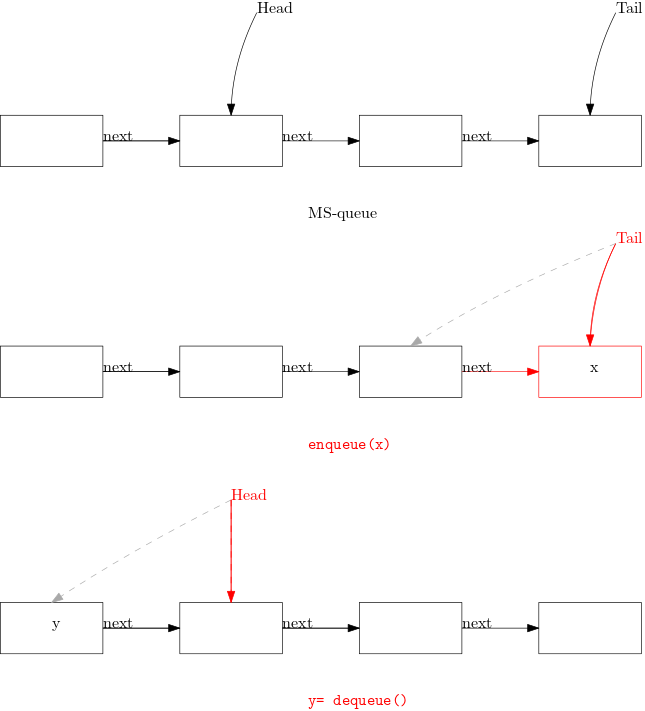
\includegraphics[scale=0.4]{pics/msqueue}
  \caption{\label{fig::msq}MS-queue structure, enqueue and dequeue operations. In the first diagram the first element has been dequeued. Red arrows show new pointers and gray dashed arrows show the old pointers.}
\end{figure}


Moir, Nussbaum, and Shalev~\cite{DBLP:conf/spaa/MoirNSS05} presented a more sophisticated queue by using the elimination technique. The elimination mechanism has the dual purpose of allowing operations to complete in parallel and reducing contention for the queue. An Elimination Queue consists of an MS-queue augmented with an elimination array. Elimination works by allowing opposing pairs of concurrent operations such as an enqueue and a dequeue to exchange values when the queue is empty or when concurrent operations can be linearized to empty the queue. Their algorithm makes it possible for long-running operations to eliminate an opposing operation. The empirical evaluation showed the throughput of their work is better than the MS-queue, but the worst case is still the same; in case there are $p$ concurrent enqueues, their algorithm is not better than MS-queue. 

Hoffman, Shalev, and Shavit~\cite{DBLP:conf/opodis/HoffmanSS07} tried to make the MS-queue more parallel by introducing the Baskets Queue. Their idea is to allow more parallelism by treating the simultaneous enqueue operations as a basket. Each basket has a time interval in which all its nodes' enqueue operations overlap. Since the operations in a basket are concurrent, we can order them in any way. Enqueues in a basket try to find their order in the basket one by one by using \texttt{CAS} operations. However, like the previous algorithms, if there are still $p$ concurrent enqueue operations in a basket, the amortized step complexity remains $\Omega(p)$ per operation.

\begin{figure}[hbt]
  \center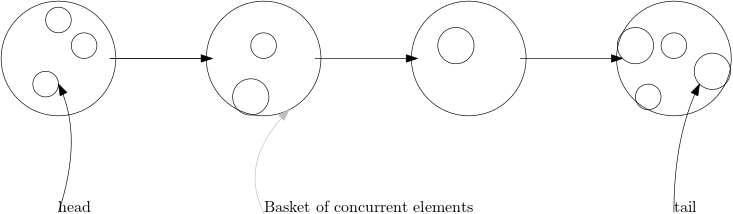
\includegraphics[scale=0.3]{pics/baskets}
  \caption{Baskets queue idea. There is a time that all operations in a basket were running concurrently, but only one has succeeded to do \texttt{CAS}. To order the operations in a basket, the mechanism in the algorithm for processes is to \texttt{CAS} again. The successful process will be the next one in the basket and so on.}
\end{figure}

Ladan-Mozes and Shavit~\cite{DBLP:journals/dc/Ladan-MozesS08} presented an Optimistic Approach to Lock-Free FIFO Queues. They use a doubly-linked list and do fewer \texttt{CAS} operations than MS-queue. But as before, the worst case is when there are $p$ concurrent enqueues which have to be enqueued one by one. The amortized worst-case complexity is still $\Omega(p)$ \texttt{CAS}es.

Hendler et al.~\cite{DBLP:conf/spaa/HendlerIST10} proposed a new paradigm called flat combining. Their queue is linearizable but not lock-free. Their main idea is that with knowledge of all the history of operations, it might be possible to answer queries faster than doing them one by one. In our work we also maintain the whole history. They present experiments that show their algorithm performs well in some situations.

Gidenstam, Sundell, and Tsigas~\cite{DBLP:conf/opodis/GidenstamST10} introduced a new algorithm using a linked list of arrays. Global head and tail pointers point to arrays containing the first and last elements in the queue. Global pointers are up to date, but head and tail pointers may be behind in time. An enqueue or a dequeue searches in the head array or tail array to find the first unmarked element or last written element (see~Figure~\ref{fig::sundell}). Their data structure is lock-free. Still, if the head array is empty and $p$ processes try to enqueue simultaneously, the step complexity remains $\Omega(p)$.

\begin{figure}[hbt]
  \center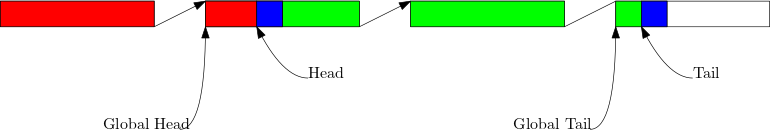
\includegraphics[scale=0.5]{pics/sundell}
    \caption{\label{fig::sundell}Global pointers point to arrays. Head and Tail elements are blue, dequeued elements are red and current elements of the queue are green.}
\end{figure}

Kogan and Petrank~\cite{DBLP:conf/ppopp/KoganP11} introduced wait-free queues based on the MS-queue and use Herlihy's helping technique to achieve wait-freedom. Their step complexity is $\Omega(p)$ because of the helping mechanism.

%todo: comparison
%Milman et al.~\cite{DBLP:conf/spaa/MilmanKLLP18} designed BQ: A Lock-Free Queue with Batching. Their idea of batching allows a sequence of operations to be submitted as a batch for later execution. It supports a new notion introduced by the authors called Extended Medium Futures Linearizability.

%Nikolaev and Ravindran~\cite{DBLP:journals/corr/abs-2201-02179} wCQ to be completed.
In the worst-case step complexity of all the list-based queues discussed above, there is a $p$ term that comes from the case all $p$ processes try to do an enqueue simultaneously. Morrison and Afek call this the \textit{CAS retry problem}~\cite{DBLP:conf/ppopp/MorrisonA13}. It is not limited to list-based queues and array-based queues share the CAS retry problem as well~\cite{DBLP:conf/spaa/TsigasZ01,DBLP:conf/icdcn/Shafiei09,DBLP:conf/iceccs/ColvinG05} . We are focusing on seeing if we can implement a queue in sublinear steps in terms of $p$ or not.

\subsection{Universal Constructions}
Herlihy discussed the possibility of implementing shared objects from other objects~\cite{10.1145/114005.102808}. A \textit{universal construction} is an algorithm that can implement a shared version of any given sequential object. We can implement a concurrent queue using a universal construction. Jayanti proved an $\Omega(\log p)$ lower bound on the worst-case shared-access time complexity of $p$-process universal constructions~\cite{DBLP:conf/podc/Jayanti98a}. He also introduced a construction that achieves $\textsc{O}(\log^2 p)$ shared accesses~\cite{DBLP:conf/podc/ChandraJT98}. His universal construction can be used to create any data structure, but its implementation is not practical because of using unreasonably large-sized \texttt{CAS} operations.

Ellen and Woelfel introduced an implementation of a Fetch\&Inc object with step complexity of $O(\log p)$ using $O(\log n$)-bit \texttt{LL/SC} objects, where $n$ is the number of operations~\cite{10.1007/978-3-642-41527-2_20}. Their idea has similarities to Jayanti's construction, and they represent the value of the Fetch\&Inc using the history of successful operations. 

%FIFO queues have a wide range of use in OS and applications. The current state-of-the-art queues are implemented using linked lists; that's why they have factor p in their time complexity.

%\href{https://docs.google.com/spreadsheets/d/1cL1tgXXdljkh462sMwkTVMHH_k0MBTmslIVM3xA5VS4/edit#gid=0}{Table of previous works}

%There is a connection between queues and universal constructions. We can implement a universal construction using a queue. We can store operations in the shared queue and compute operations' responses using the queue's content. Some impractical universal constructions are using big words as "...".
\section{Adiitional ones}
\subsection{Tsigas and Zhang}
Tsigas and Zhang \cite{DBLP:conf/spaa/TsigasZ01} present a cyclic array queue that allows the head and tail to lag at most m nodes behind the actual head and tail of the queue, so the amortized number of CAS executions per operation is 1 + 1/m. Their algorithm is limited to bounded queues due to their static allocation.

\subsection{Kogan and Herlihy}
Previous works present concurrent constructs that combine multiple operations into a single operation on the shared object. We chose to combine operations and apply them as batches, to increase scalability. The work of Kogan and Herlihy \cite{DBLP:conf/podc/KoganH14} is the closest to this work. They propose alternative definitions for linearizability of executions with batches, including MF-linearizability, which we use. They describe very simple implementations of stacks, queues, and linked lists that demonstrate the benefits of using futures.



\subsection{Yang and Mellor-Crummey}
Because of the problem of failure of CASes one way is to use other primitive objects other than CAS objects. Yang and Mellor-Crummey \cite{DBLP:conf/ppopp/YangM16} utilize fetch-and-add as well, to form a wait-free queue.  They present the first linearizable and wait-free FIFO queue based on fetch-and-add (FAA). While compare-and-swap (CAS) based non-blocking algorithms may perform poorly due to work wasted by CAS failures, algorithms that coordinate using FAA, which is guaranteed to succeed, can in principle perform better under high contention. 

I could not compute its complexity but I guess it is hard or not important

\bibliography{main} 

\end{document}

